\section{Quantum error coorection}

It's perfectly known how computers are affected from machine errors, where bits can possibly change states due to various external factors. The same thing happens to quantum computers, in paticular qubits are much more delicate having a greate number of possible fluctuations that needs to be taken into account when we run an algorithm. Therefore, we need to create protocols that allow us to correct such variations of the state during the computations as we have inside classical computers. In order to understand how this can be done on a quantum level is really usefull to see its classical version and grasp the major concepts to use also on quantum computers.

On classical computers a bit can change state randomically going from $0$ to $1$ or viceversa with a certain probability $p$ inside the circuit. Such a situation define a particular type of transformation that we will define as follows.
\dfn{Binary symmetric channel}
{
    When we will have a transformation $X:\{0,1\} \to \{0,1\}$ acting on the state of a logic variable so that $X(0) = 1$ with a certain probability $p$ and $X(0) = 0$ with $1-p$ it's called binary symmetric channel.
}
\noindent
Such are the randomic trasnformation that acts on the single bits inside a normal computer, having that they can be overcomed using a regular routine that has becomed standard over the years. The idea is the following, we are going to \textbf{encode} the state of a single bit using three of them such as follows
\begin{align}
    &0 \mapsto 000, &1\mapsto 111.
\end{align}
In this way we will have that an error on one the bits defining the state can be \textbf{dyagnosed} by looking at the other two. In particular, we will have that if we start from $000$ and on the line we see a $100$ we know that an error has occoured, and we are able to correct it. We know how the possible flips that could have happened bringing to the $100$ are: a flip to the first bit in the state $000$, and two bits flips for second and third in the $111$ state. In this context, in order to \textbf{recover} the state, the idea is to return to the state that has the higher probability of being the right one, in the situation we have discussed is the $000$ since we have a probability $p$ of flipping to that state while $111$ has a probability $p^2$. Such a protocol, called \textbf{majority rate}, allows to brign the possibility of the error to propagate inside the circuit to the one given by the following result.
\thm{Majority rate error probability}
{
    The probability of committing an error by using the majority rate protocol is given by
    \begin{equation}
        \label{eq:ErrMajoRate}
        p_{err} = 3p^2 - 2p^3.
    \end{equation}
}
\pf{Proof}
{
    In the protocol we are basically ignoring the possibilities of having more than one flip, so tha tthe error is given by the possibility of having every two flip or a three bit flip, giving
    \begin{equation}
        p_{err} = 3p^2(1-p) + p^3 = 3p^2 - 2p^3.
    \end{equation}
}
\noindent
It's also interesting to see how such a simple protocol is also not always usefull. In fact, the inequality $3p^2 - 2p^3 < p$ is true only if $p < 1/2$ or the opposite is real, having that such an error correction can be used only if the probability of error of a single bit is already bellow that threshold.

This was a simple protocol, but it still shows the main important features that a general error correction code should have in principle. We can sintetyze what is needed in order to correct the error on an abstract level as: encoding of the state, dyagnosis of the error committed, and recover of the original state. All of this is not difficult to imagine done inside a normal computer, still working with quantum information makes thing a lot harder due to the presence of some complications:
\begin{enumerate}[label*=\protect\fbox{\arabic{enumi}}]
    \item The no cloning theorem makes diffucult coping the state, having that encoding is not too much straightforward;
    \item The types of errors inside a qubit are larger than the simple flip of a bit, in fact we have the whole range of continuos unitary transformation to span;
    \item Recover a state it's not easy to do expecially remembering that if we measure a state we are going to lose it forever.
\end{enumerate}
Nevertheless, we will show step by step how such a task can still be brought up generating an error correction protocol that allows to save qubits information to be currupted in the process.

\subsection{Single qubit flip errors}

To start this journey we shall look into the simplest case of quantum error that we can imagine, the quantum version of the bit flip. Assume that there's a probability $p$ that a gate $X$ is applied to the state $\ket{\psi}$ of the qubit inside the cirtuit. One shall recall how the $X$ gate acts as a NOT inside a quantum cirtuit generating a flip of the $\ket{0}$ and $\ket{1}$ gates. In this way we can imagine to work exactly as in the classical case and start by encoding the states using three qubits so that a general state becomes
\begin{equation}
    \label{eq:baseState}
    \ket{\psi} = a\ket{0} + b\ket{1} \mapsto a \ket{000} + b \ket{111} = \ket{\psi_0}.
\end{equation}
Therefore, we shall start by understanding how to effectivelly do this, and the answer is easier than it seems thanks to the use of two CNOT as described in \figref{fig:SinQuEncod}.
\begin{figure}[t]
    \centering
    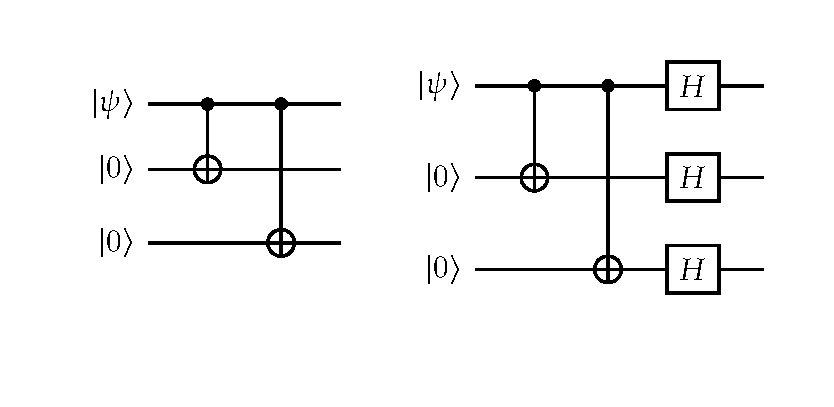
\includegraphics[width=0.8\textwidth]{Immagini/SinQuEncod.pdf}
    \caption{
        Encoder circuit for the simple single qubit error correction routines, in particular the one on the left is the one for the state flip while on the right there's the one for the phase flip.
    }
    \label{fig:SinQuEncod}
\end{figure}
The first circuit reported on the left of that figure creates a gate, that we will call $E$, that perform exactly the wanted operation. In this way the first step is performed, now we shall be able to understand if a state flip error happens by the fact that $\ket{\psi_0}$ will change state going from \eqref{eq:baseState} to one of the following
\begin{equation}
    \label{eq:FlippedStates}
    \ket{\psi_1} = a\ket{100} + b \ket{011}, \hspace{1cm} \ket{\psi_2} = a\ket{010} + b\ket{101}, \hspace{1cm} \ket{\psi_3} = a\ket{001} + b\ket{110}.
\end{equation}
The last thing that we need to understand is how we can understand in which state is the system in order to then correct it. The idea is so to mesure the state using a particular mesure defined as
\begin{align}
    &\{\hat{P}_k\}_{k=0}^3, &\hat{P}_k = \ketbra{\psi_k},
\end{align}
which will allow us to mesure exactly which state we have whithout making it collapse. In fact, if we are in a state $\ket{\psi_j}$ we will have that
\begin{equation}
    p_k = \ev{\hat{P}_k}{\psi_j} = \begin{cases}
        0 & j \neq k\\
        \abs{a}^2 + \abs{b}^2 & j = k
    \end{cases} = \delta_{jk},
\end{equation}
meaning that the only possible state in which $\ket{\psi_j}$ can collapse into is itself. This will allow us to evaluate the state perfectly giving a good diagnose of the error that has occured, a mesure that allow us to do this is called \textbf{syndrome operator}. Subsequently, after understand the state of the system, we will be able to correct the error by appling an $X$ operator on the flipped qubit.


To make an example of such measure different from the projector theoretical one, we can simply define it by using a series of $Z$ operators. We remember how $\ket{0}$ and $\ket{1}$ are the eigenstates of the operator so that $Z\ket{0/1} = +1/-1\ket{0/1}$. Knowing it we can define the operators
\begin{equation}
    Z_1Z_2 = Z_1\otimes Z_2\otimes \mathbb{1}_3 = [+1(\ketbra{00} + \ketbra{11}) -1(\ketbra{10} + \ketbra{01})]\otimes \mathbb{1}_3,
\end{equation}
which shows how it returns $+1$ if the first and second qubit are equal, and $-1$ otherwise. In this way we can define a really clever syndrome opeartor measure by using only two operators $Z_1Z_2$ and $Z_2Z_3$, having that by their value we can understand the error exactly. In fact, by knowing which qubits are equal or not allows us to tell exactly which of the four state we have in that specific moment.

This method is so an exact copy of the classical one setted in a quantum environment, and we can see how it is the same as before since the probability of an error to propagate using this routine is given exactly by \eqref{eq:ErrMajoRate}. Meaning that this can be implemented only if the error rate is already below the $50\%$, but still this is a good simple algorithm since can be applied not only to the case of the state flip but also to other type of errors. For example, for a qubit not only the state can be change by external factor, but also the phase is vulnerable. In particular, we can imagine that now the operator that is applied with a probability $p$ is $Z$, which applied on $\ket{\psi}$ will flip the phase of $\ket{1}$. One may think that such an error needs to be trated differently from the one seen before, but that would be not true. In fact, we can see how if instead of the computational base we use $\ket{\pm}$ to represent the states the problem returns to a flip of the state since $Z\ket{\pm} = \ket{\mp}$. Therefore, if we encode the states by using the circuit in \figref{fig:SinQuEncod} that performs the following tranformation
\begin{align}
    &\ket{0}\mapsto \ket{+++}, &\ket{1}\mapsto\ket{---},
\end{align}
we can then define the syndrome mesure by also changin base as the normal one and obtaining
\begin{equation}
    H^{\otimes 3} Z_1Z_2 H^{\otimes 3} = X_1X_2. 
\end{equation}
This will allow us to understand if a phase flip happens allowing us to recover the initial state without any problem, reducing the probability of error as seen before.

\subsection{Shor code}

We have seen how we are able to correct both states flips and phase flips in a separate way, but inside a quantum computer we are interested in the full correction of the qubits aiming to a protocol allowing for the correction of both at the same time. Such a routine exist and is called \textbf{Shor code} that we shall see next.

The idea starts with the encoding of the states by using a total of $9$ qubits mapping the computational base to the following monsters
\begin{align}
    &\ket{0} = \left( \frac{\ket{000} + \ket{111}}{\sqrt{2}} \right)_{B1}\left( \frac{\ket{000} + \ket{111}}{\sqrt{2}} \right)_{B2}\left( \frac{\ket{000} + \ket{111}}{\sqrt{2}} \right)_{B3} = \ket{+}_{B1}\ket{+}_{B2}\ket{+}_{B3},\\
    &\ket{1} = \left( \frac{\ket{000} - \ket{111}}{\sqrt{2}} \right)_{B1}\left( \frac{\ket{000} - \ket{111}}{\sqrt{2}} \right)_{B2}\left( \frac{\ket{000} - \ket{111}}{\sqrt{2}} \right)_{B3} = \ket{-}_{B1}\ket{-}_{B2}\ket{-}_{B3}.
\end{align}
Basically defining three blocks with inside the same encoded state of before, having in fact an encoder circuit really close to the two seen previously as depicted in \figref{fig:ShorEncoder}.
\begin{figure}[t]
    \centering
    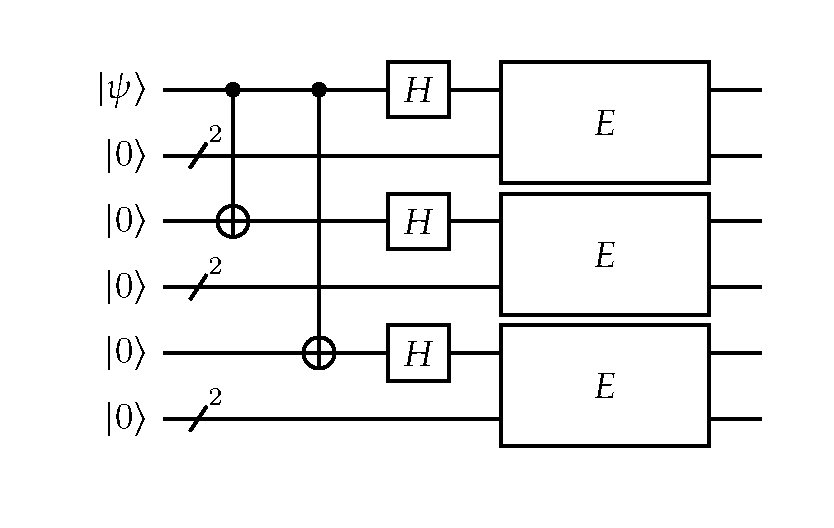
\includegraphics[width=0.8\textwidth]{Immagini/ShorEncoder.pdf}
    \caption{
        Encoder for the Shor code, where the gates defined by $E$ are ncoders for the simple case of the state flip correction.
    }
    \label{fig:ShorEncoder}
\end{figure}
Now, we can go and see what happens if we have a state or phase flip inside one of the qubit. In the case of the state flip, we can see how one of the blocks will change the state as in \eqref{eq:FlippedStates} so that we can use a generalization of the $Z_1Z_2$ measure to find out the error
\begin{equation}
    Z_1Z_2 = (Z_1Z_2)_{B1}\otimes\mathbb{1}_{B2}\otimes\mathbb{1}_{B3}.
\end{equation}
We have so an efficient way to spot the state errors and correct them by simply apply a NOT where needed. Then, for the phase flips instead we will have that one of the blocks will change having that $\ket{\pm}$ will fo into $\ket{\mp}$. To spot which one of the blocks we need to correct we can use the same idea seen previously for the phase flip, where we can use the following operators
\begin{align}
    &S_1 = X_{B1}X_{B2} = (X_1X_2X_3)\otimes(X_4X_5X_6)\otimes\mathbb{1}_{B3},\\
    &S_2 = X_{B2}X_{B3} = \mathbb{1}_{B1} \otimes (X_4X_5X_6)\otimes (X_7X_8X_9).
\end{align}
In this way we can be sure to see every possible state and phase flip inside our circuit and be able to correct them properly. That was all we needed in our machines, in fact we can see how every possible error can be described in terms of those two primitive problems as follows.
\thm{Universality of Shor code}
{
    Every possible error inside quantum computers can be decomposed in phase and state flips, so that Shor code forms a universal error correcting procedure.
}
\pf{Proof}
{
    In order to prove that we will need some notions from the theory of open systems. Meaning that inside the context of SE evolution the state is preserved, and no random error should occure all is deterministic. Still, when the system is coupled with environment random change in the state can appear and $\ket{\psi}$ evolves from a pure state to a mixed one. Such evolution can be described by a more general version of the dynamic equation called \textbf{Lindblad equation} which is well known, and shows an evolution that can be described by a \textbf{quantum channel} acting as follows
    \begin{equation}
        \ket{\psi} \mapsto \sum_i E_i^\dagger \ketbra{\psi} E_i.
    \end{equation}
    Where, $E_i$ is a set of operators with the property of being complete meaning $\sum_i E_i^\dagger E_i = \mathbb{1}$, condition needed in order to conserve the norm of the state. Now, we can imagine having a $1$-qubit situation so that $E_i$ are $2\times 2$ matrices and therefore can be written as expansion of the Pauili matrices base as
    \begin{equation}
        E_i = e_0\mathbb{1} + e_1 X + e_2Y + e_3Z.
    \end{equation}
    We can interprete this result by seing how the part with $\mathbb{1}$ gives out the normal evolution, the SE like one with no errors, while all the others describe possible evolution when \textbf{decoherence}, errors, occours. In particular, we can see that the possible errors are given by the state flip, the $X$ part, phase flip, the $Z$, and the $Y$ one that can be written as $ZX$ giving rise to a situation when both occours. Therefore, all possible errors are linear combinations of the primitive ones that Shor code can predict and cure.
}